%%%%%%%%%%%%%%%%%%%%%%%%%%%%%%%%%%%%%%%%%
% Short Sectioned Assignment
% LaTeX Template
% Version 1.0 (5/5/12)
%
% This template has been downloaded from:
% http://www.LaTeXTemplates.com
%
% Original author:
% Frits Wenneker (http://www.howtotex.com)
%
% License:
% CC BY-NC-SA 3.0 (http://creativecommons.org/licenses/by-nc-sa/3.0/)
%
%%%%%%%%%%%%%%%%%%%%%%%%%%%%%%%%%%%%%%%%%

%----------------------------------------------------------------------------------------
% PACKAGES AND OTHER DOCUMENT CONFIGURATIONS
%----------------------------------------------------------------------------------------

\documentclass[paper=a4, fontsize=11pt]{scrartcl} % A4 paper and 11pt font size

\usepackage[T1]{fontenc} % Use 8-bit encoding that has 256 glyphs
\usepackage{fourier} % Use the Adobe Utopia font for the document - comment this line to return to the LaTeX default
\usepackage[norsk]{babel} 
\usepackage[utf8]{inputenc}
\usepackage{amsmath,amsfonts,amsthm} % Math packages
\usepackage{tikz} % drawing package
\usepackage{hhline}

\usepackage{sectsty} % Allows customizing section commands
\allsectionsfont{\centering \normalfont\scshape} % Make all sections centered, the default font and small caps

\usepackage{pdfpages}

\usepackage{fancyhdr} % Custom headers and footers
\pagestyle{fancyplain} % Makes all pages in the document conform to the custom headers and footers
\fancyhead{} % No page header - if you want one, create it in the same way as the footers below
\fancyfoot[L]{} % Empty left footer
\fancyfoot[C]{} % Empty center footer
\fancyfoot[R]{\thepage} % Page numbering for right footer
\renewcommand{\headrulewidth}{0pt} % Remove header underlines
\renewcommand{\footrulewidth}{0pt} % Remove footer underlines
\setlength{\headheight}{13.6pt} % Customize the height of the header

\numberwithin{equation}{section} % Number equations within sections (i.e. 1.1, 1.2, 2.1, 2.2 instead of 1, 2, 3, 4)
\numberwithin{figure}{section} % Number figures within sections (i.e. 1.1, 1.2, 2.1, 2.2 instead of 1, 2, 3, 4)
\numberwithin{table}{section} % Number tables within sections (i.e. 1.1, 1.2, 2.1, 2.2 instead of 1, 2, 3, 4)

\setlength\parindent{0pt} % Removes all indentation from paragraphs - comment this line for an assignment with lots of text

%---- Listings --------------
\usepackage{color}
\definecolor{light-gray}{gray}{0.95}
\usepackage{listings}

\lstset{ %
language=C,                     % choose the language of the code
basicstyle=\footnotesize,       % the size of the fonts that are used for the code
numbers=left,                   % where to put the line-numbers
numberstyle=\footnotesize,      % the size of the fonts that are used for the line-numbers
stepnumber=1,                   % the step between two line-numbers. If it is 1 each line will be numbered
resetmargins=true,              % reset line numbers
numbersep=5pt,                  % how far the line-numbers are from the code
backgroundcolor=\color{white},  % choose the background color. You must add \usepackage{color}
showspaces=false,               % show spaces adding particular underscores
showstringspaces=false,         % underline spaces within strings
showtabs=false,                 % show tabs within strings adding particular underscores
frame=single,                   % adds a frame around the code
tabsize=2,                      % sets default tabsize to 2 spaces
captionpos=b,                   % sets the caption-position to bottom
breaklines=true,                % sets automatic line breaking
breakatwhitespace=false,        % sets if automatic breaks should only happen at whitespace
escapeinside={\%*}{*)}          % if you want to add a comment within your code
}

%----------------------------------------------------------------------------------------
% TITLE SECTION
%----------------------------------------------------------------------------------------

\newcommand{\horrule}[1]{\rule{\linewidth}{#1}} % Create horizontal rule command with 1 argument of height

\title{ 
\normalfont \normalsize 
\textsc{TDT4205 Compilers, NTNU} \\ [25pt] % Your university, school and/or department name(s)
\horrule{0.5pt} \\[0.4cm] % Thin top horizontal rule
\huge Problem Set 3 \\ % The assignment title
\horrule{2pt} \\[0.5cm] % Thick bottom horizontal rule
}

\author{Christoffer Tønnessen \& Stian Jensen} % Your name

\date{\normalsize\today} % Today's date or a custom date

\begin{document}

\maketitle % Print the title

%----------------------------------------------------------------------------------------
% PROBLEM 1
%----------------------------------------------------------------------------------------
\section{Parsing}
%----------------------------------------------------------------------------------------
\subsection{Part a)}
When you parse a string in regards to a grammar there are two main ways of constructing the parsing tree. One technique is called top-down parsing and the other bottom-up.

A top-down parser uses the non-terminals of the grammar as the basis for the parsing. It starts on the start symbol of the grammar and works its way down the parse tree by changing the non-terminals one at a time. The parser might do a lot of backtracking. To test all possibilities one eveutally would need exponential memory space. This technique might need a look-a-head to work properly.

As opposed to top-down parsing, bottom-up uses the terminals of the input string as basis for the parsing. One at a time it checks the next token of the input. It changes continously the input to tokens based on the grammar. When it hits the start symbol, it's done. Just like the top-down parsing technique the parser might need a look-a-head to be sure to work.
%----------------------------------------------------------------------------------------
\subsection{Part b)}
An LL parser is a top-down parser for the subset of context-free grammars. LL stands for left to right, leftmost derivation. An LL parser has two actions: \textit{predict} that chooses which production that needs to be applied to get closer to the goal and \textit{match} that matches the leftmost guessed terminal symbol with the leftmost unconsumed symbol of input.

An LR parser is a bottom-up parser that efficiently handle deterministic context-free garmmars in guaranteed linear time. LR stands for left to right, rightmost derivation. An LR parser has two actions: \textit{shift}, which adds the next token of input to the buffer and \textit{reduce} that reduces the colleciton of terminals and non-terminals back to a terminal by reversing a production.
%----------------------------------------------------------------------------------------
% PROBLEM 2
%----------------------------------------------------------------------------------------
\section{Top-down parsing}
%----------------------------------------------------------------------------------------
\subsection{Part a)}
\begin{center}
    \begin{tabular}{ | l | l | }
    \hline
    First sets                              & Follow sets                   \\
    \hline
    FIRST(A) = \{ a, b, c, d, e, f \}       & FOLLOW(A) = \{ \$ \}          \\
    \hline
    FIRST(B) = \{ b \}                      & FOLLOW(B) = \{ e, c, f, \$ \} \\
    \hline
    FIRST(C) = \{ b, $\epsilon$ \}          & FOLLOW(C) = \{ e, c, f, \$ \} \\
    \hline
    FIRST(D) = \{ b, d, e \}                & FOLLOW(D) = \{ \$ \}          \\
    \hline
    FIRST(E) = \{ e, $\epsilon$ \}          & FOLLOW(E) = \{ b, c, f \}     \\
    \hline
    FIRST(F) = \{ c, f \}                   & FOLLOW(F) = \{ \$ \}          \\
    \hline
    \end{tabular}
\end{center}
A is put as the start symbol in this grammar.
%----------------------------------------------------------------------------------------
\subsection{Part b)}
\begin{center}
    \begin{tabular}{ | l || l | l | l | l | l | l | l | }
    \hline
        & a         & b             & c             & d         & e             & f                 &   \$              \\
    \hhline{|=||=|=|=|=|=|=|=|}
    A   & A->aB     & A-D           & A->F          & A->D      & A->D          & A->F              &                   \\
    \hline
    B   &           & B->bC         &               &           &               &                   &                   \\
    \hline
    C   &           & C->bC         & C->$\epsilon$ &           & C->$\epsilon$ & C->$\epsilon$     & C->$\epsilon$     \\
    \hline
    D   &           & D->EB         &               & D->dBEF   & D->EB         &                   &                   \\
    \hline
    E   &           & E->$\epsilon$ & E->$\epsilon$ &           & E->e          & E->$\epsilon$     &                   \\
    \hline
    F   &           &               & F->c          &           &               & F->f              &                   \\
    \hline
    \end{tabular}
\end{center}
%----------------------------------------------------------------------------------------
\subsection{Part c)}
\begin{center}
    \begin{tabular}{ | l | l | l | l | }
    \hline
    Stack       & Matched part      & Remaining     & Action taken          \\
    \hhline{|=|=|=|=|}
    A\$         &                   & dbbbf         &                       \\
    \hline
    D\$         &                   & dbbbf         & A->D                  \\
    \hline
    dBEF\$      & d                 & bbbf          & D->dBEF               \\
    \hline
    BEF\$       &                   & bbbf          & match                 \\
    \hline
    bCEF\$      & b                 & bbf           & B->bC                 \\
    \hline
    CEF\$       &                   & bbf           & match                 \\
    \hline
    bCEF\$      & b                 & bf            & C->bC                 \\
    \hline
    CEF\$       &                   & bf            & match                 \\
    \hline
    bCEF\$      & b                 & f             & C->bC                 \\
    \hline
    CEF\$       &                   & f             & match                 \\
    \hline
    EF\$        &                   & f             & C->$\epsilon$         \\
    \hline
    F\$         &                   & f             & E->$\epsilon$         \\
    \hline
    f\$         & f                 &               & f->f                  \\
    \hline
    \$          &                   &               & match                 \\
    \hline
                &                   &               & \em{accept}           \\
    \hline
    \end{tabular}
\end{center}
%----------------------------------------------------------------------------------------
% PROBLEM 3
%----------------------------------------------------------------------------------------
\section{Button-up parsing}
%----------------------------------------------------------------------------------------
\subsection{Part a)}
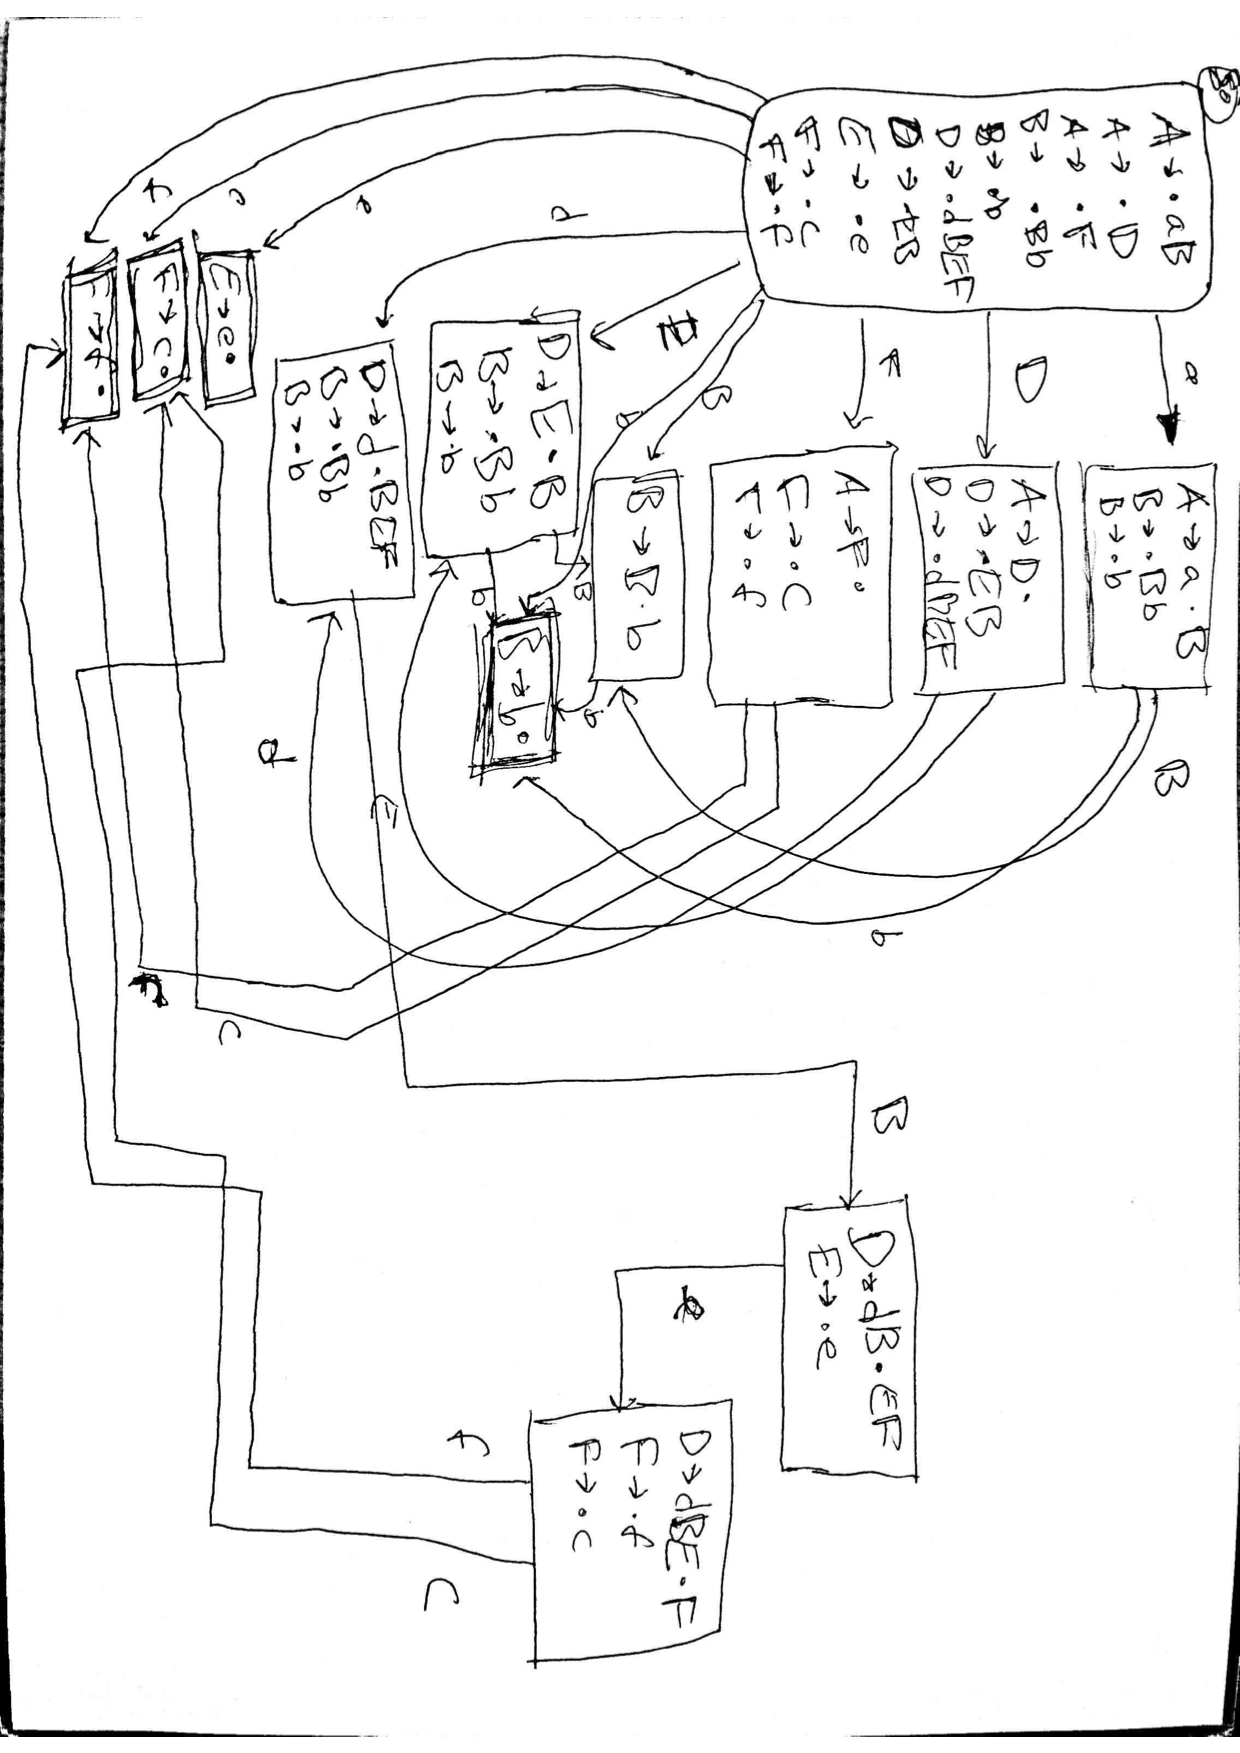
\includegraphics[scale=.65]{oppg_3a.png}
%----------------------------------------------------------------------------------------
\subsection{Part b)}
%----------------------------------------------------------------------------------------
\subsection{Part c)}
%----------------------------------------------------------------------------------------
\end{document}
